\chapter{Сравнение производительности алгоритмов}

В теории игр сравнивать разные алгоритмы достаточно просто - можно посмотреть на награды, полученные алгоритмами за эпизод.
Дополнительных метрик и критериев для сравнения не требуется.

Для начала убедимся в необходимости использовать специальные алгоритмы для сред с несколькими агентами.
На рисунке \ref{aboba} \cite{https://doi.org/10.48550/arxiv.1509.02971} представлены награды за эпизод следующей игры: один агент говорит другому точку, в которую нужно бежать, а другой агент бежит в эту точку (на время).
Видно, что классические алгоритмы не способны понять необходимость кооперации.


\begin{figure}[H]
	\centering
	\begin{subfigure}[b]{0.45\textwidth}
		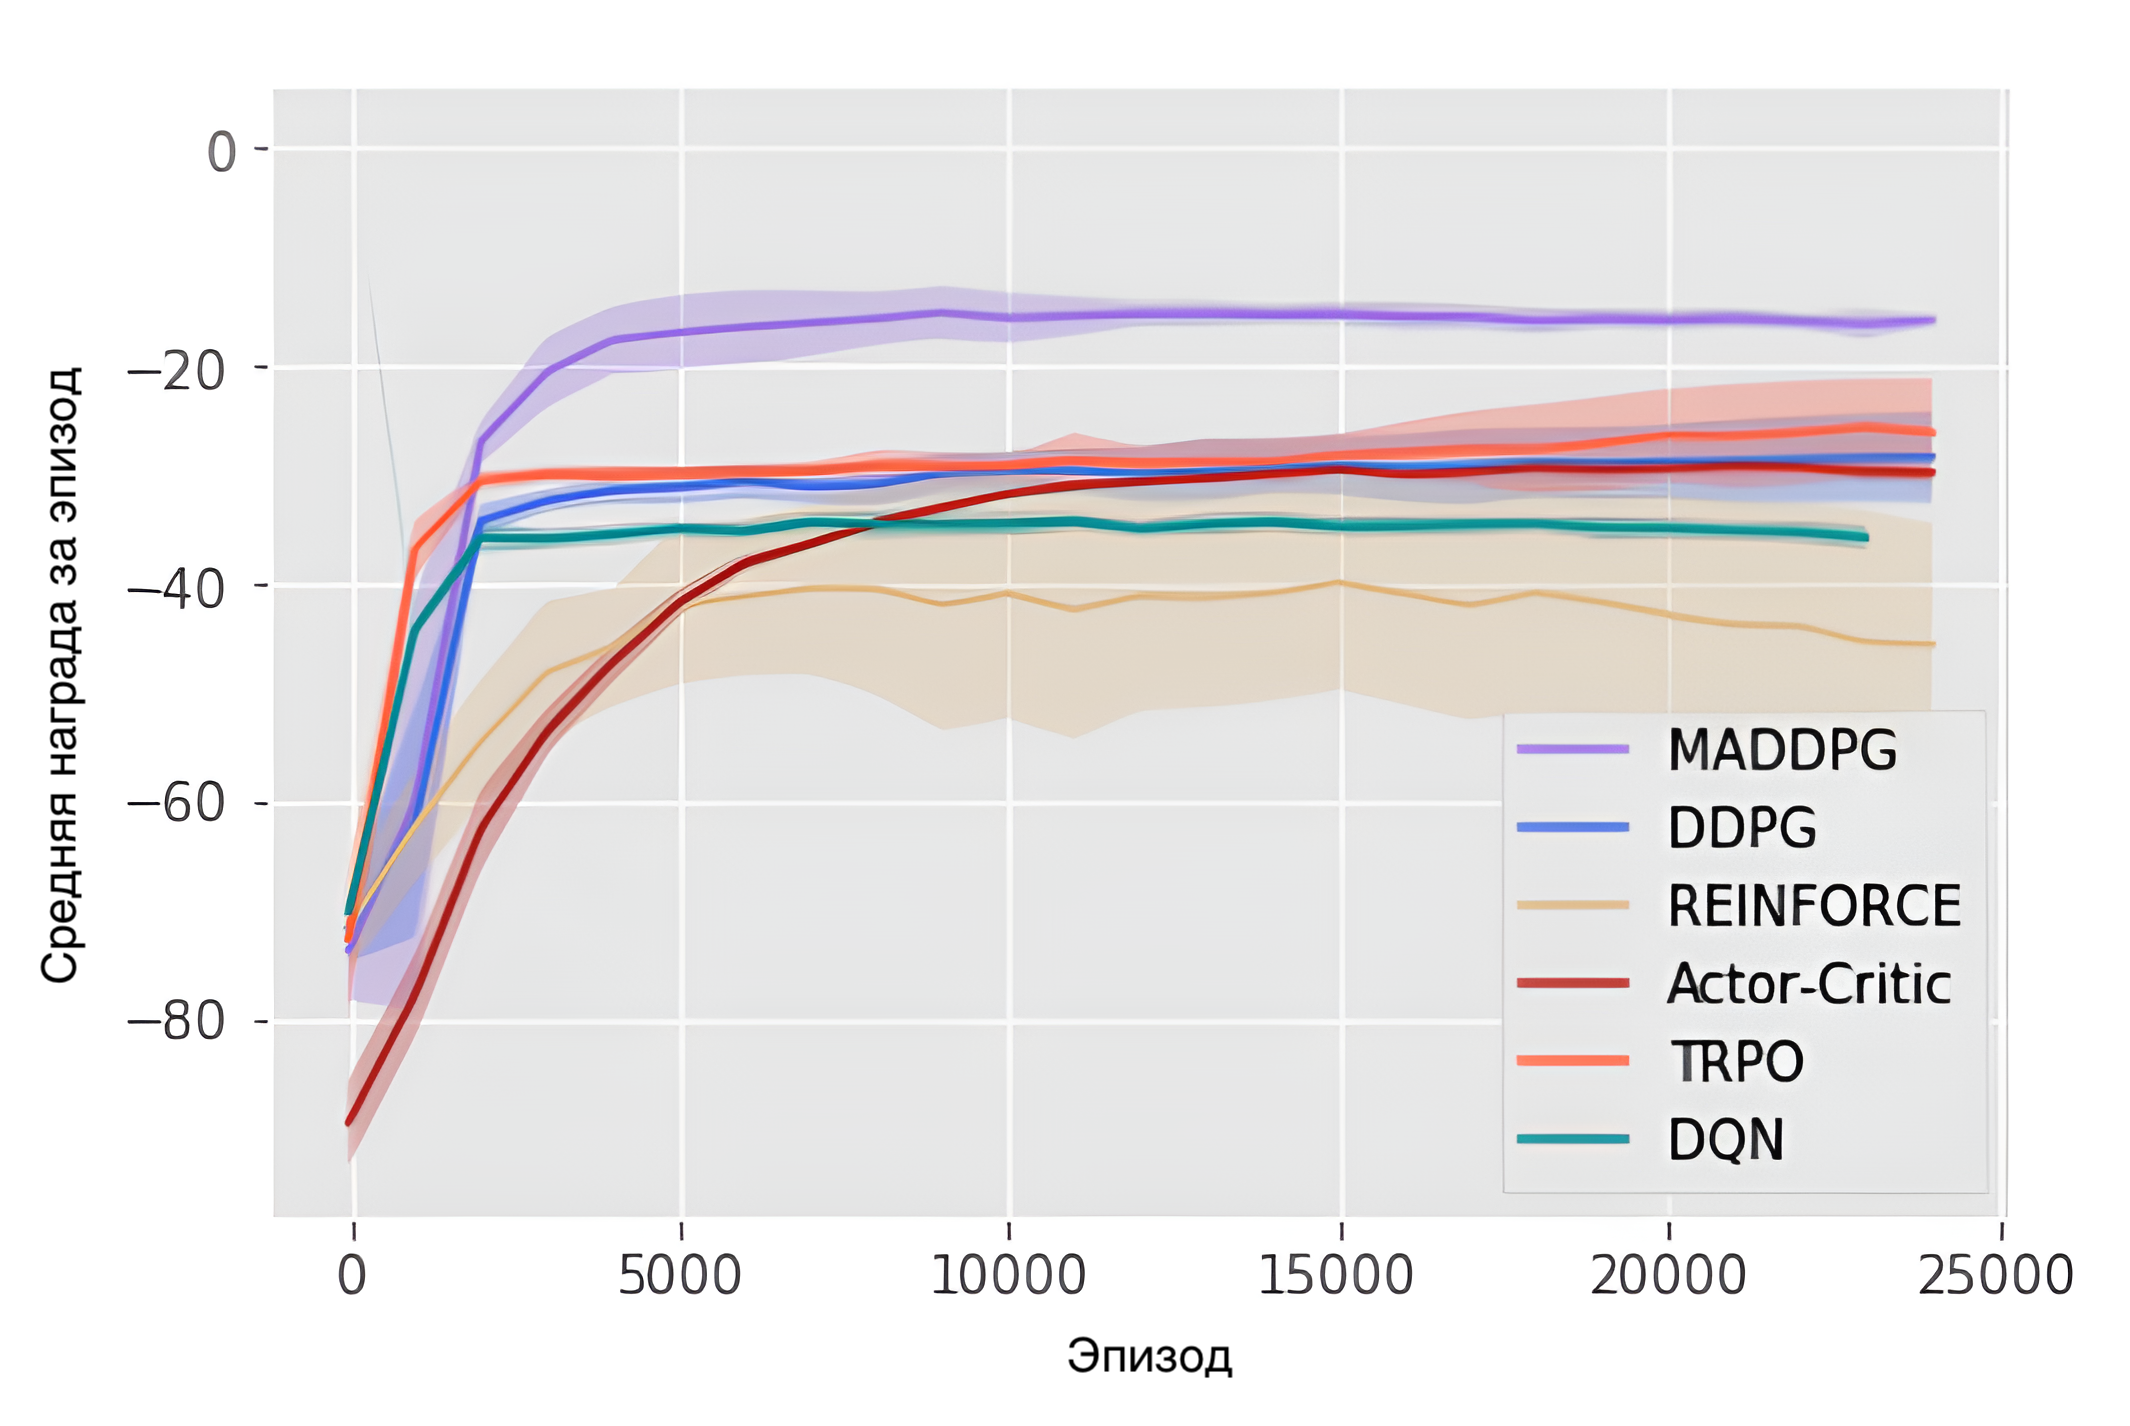
\includegraphics[width=\textwidth]{./inc/img/rl_vs_marl.png}
		\caption{Средняя награда за эпизод}
	\end{subfigure}
	\hfill
	\begin{subfigure}[b]{0.45\textwidth}
		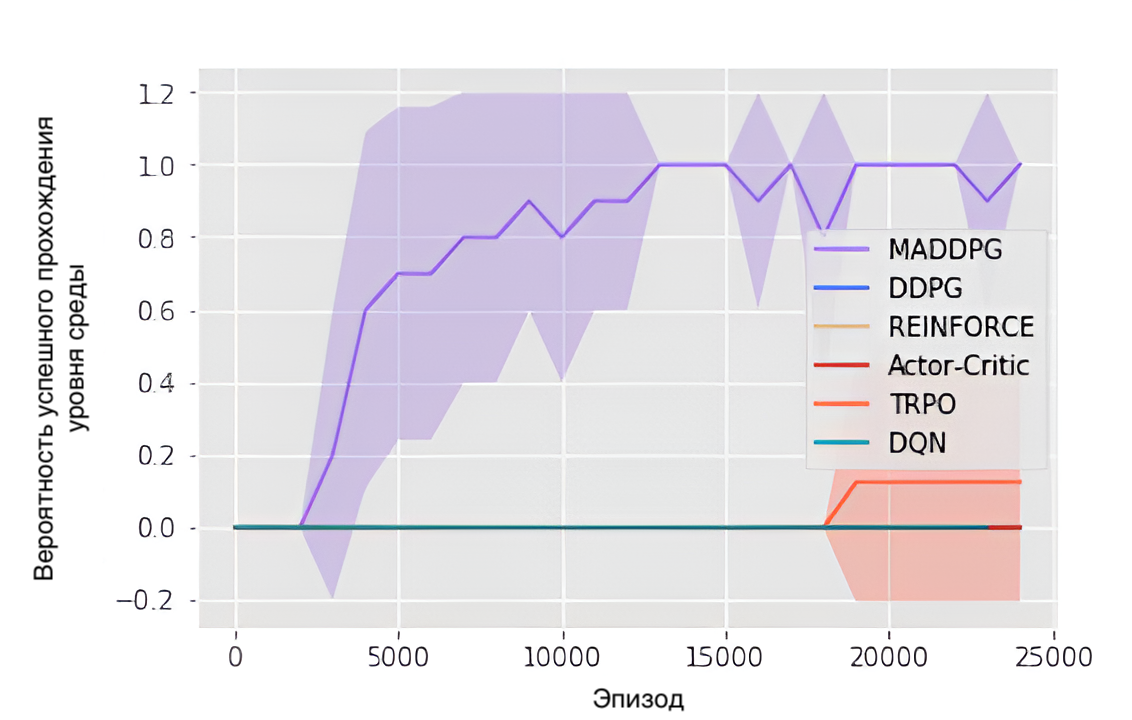
\includegraphics[width=\textwidth]{./inc/img/rl_vs_marl_2.png}
		\caption{Процент ситуаций, когда агент достигает цели}
	\end{subfigure}
		\caption{\centering Сравнение производительности MARL алгоритма MADDPG и классических RL алгоритмов}
	\label{aboba}
\end{figure}



\begin{figure}[H]
	\begin{center}
	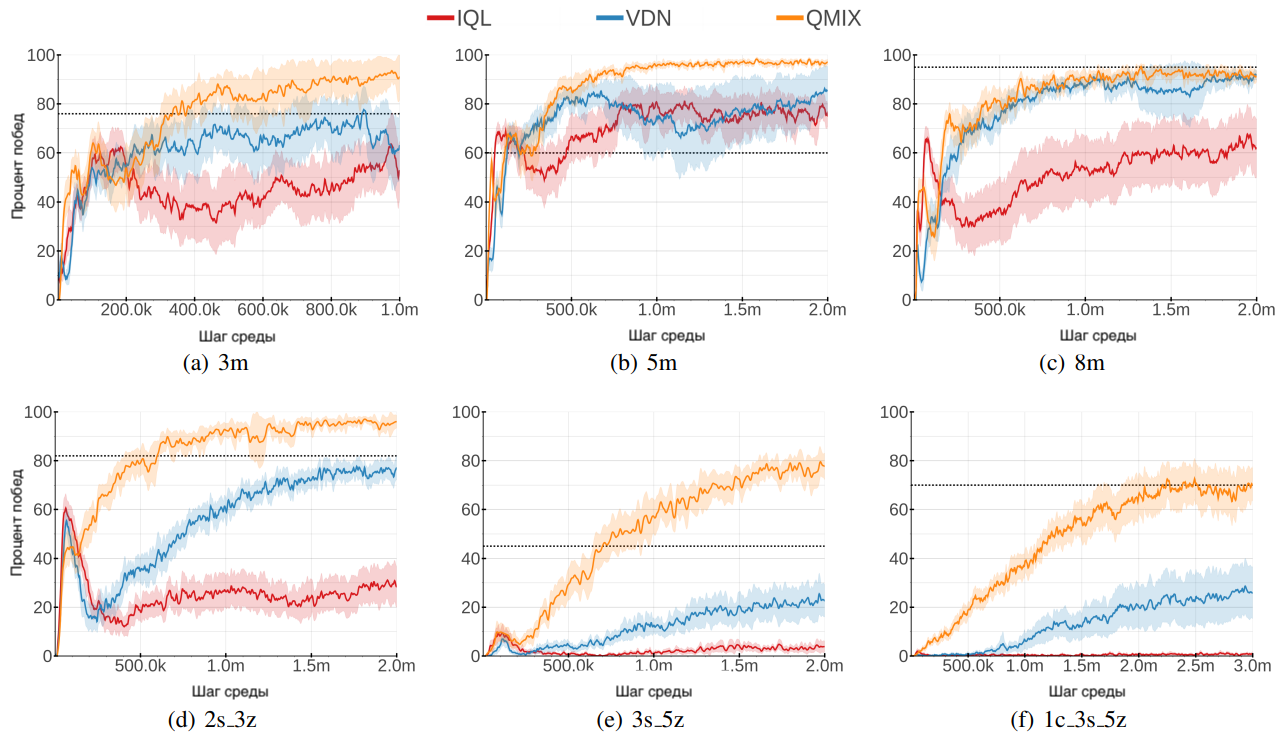
\includegraphics[pages=-, width=140mm]{./inc/img/qmix_winrate.png}
	\caption{Сравнение процента побед QMIX, VDN, IQL в среде StarCraft II в зависимости от кол--ва эпизодов для обучения}
	\label{fig:qmix_winrate}
\end{center}
\end{figure}

Алгоритмы COMA, QTRAN очень похожи на QMIX, и их рассмотрение избыточно. Таким образом, они показывают практически нулевой результат, по сравнению рассмотренными алгоритмами на \ref{fig:maven_winrate} \cite{DBLP:journals/corr/abs-1910-07483}.

\begin{figure}[H]
	\begin{center}
	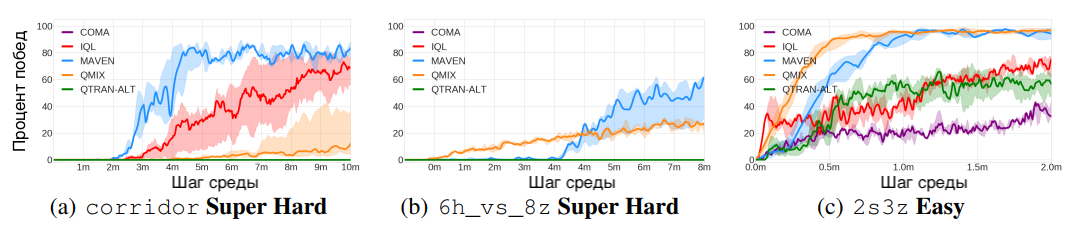
\includegraphics[pages=-, width=140mm]{./inc/img/maven_winrate.png}
	\caption{Сравнение процента побед MAVEN, QMIX, IQL, COMA, QTRAN, в среде StarCraft II в зависимости от кол--ва эпизодов для обучения}
	\label{fig:maven_winrate}
\end{center}
\end{figure}

Видно, что MAVEN и QMIX лидируют во всех категориях. Особенно хорошо использовать MAVEN в среде SMAC(StarCraft II), т. к. пространство действий в ней очень большое и необходимо его консистентно исследовать \cite{DBLP:journals/corr/abs-1910-07483}.

%\begin{figure}[H]
%	\begin{center}
%	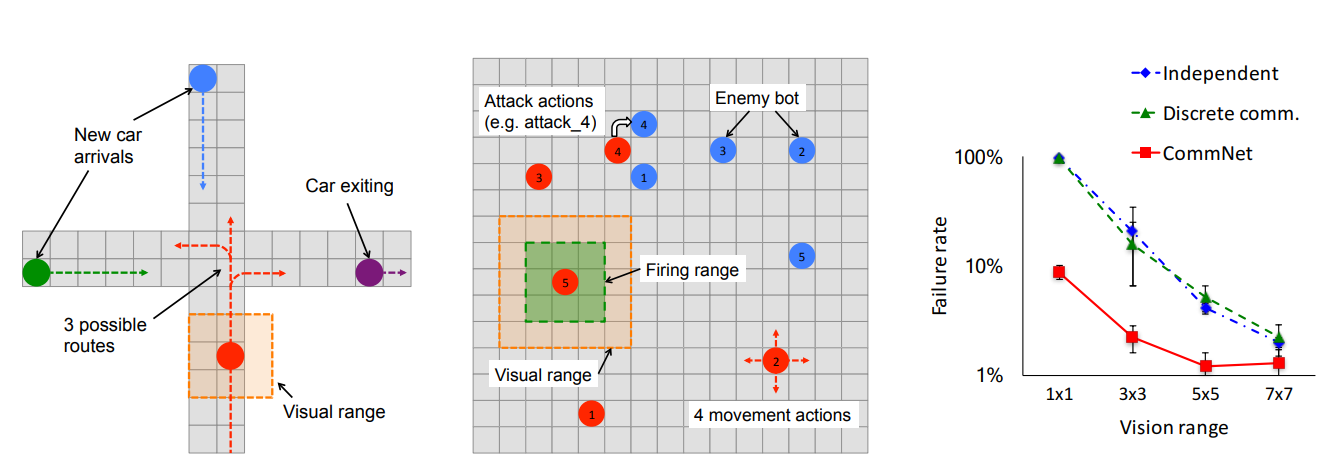
\includegraphics[pages=-, width=140mm]{./inc/img/commnet_perf.png}
%	\caption{Процент неудач в среде CrossRoad (слева) в зависимости от поля видимости для агентов управляемых независимыми сетями и алгоритмом CommNet}
%	\label{fig:commnet_perf}
%\end{center}
%\end{figure}

\begin{figure}[H]
	\begin{center}
	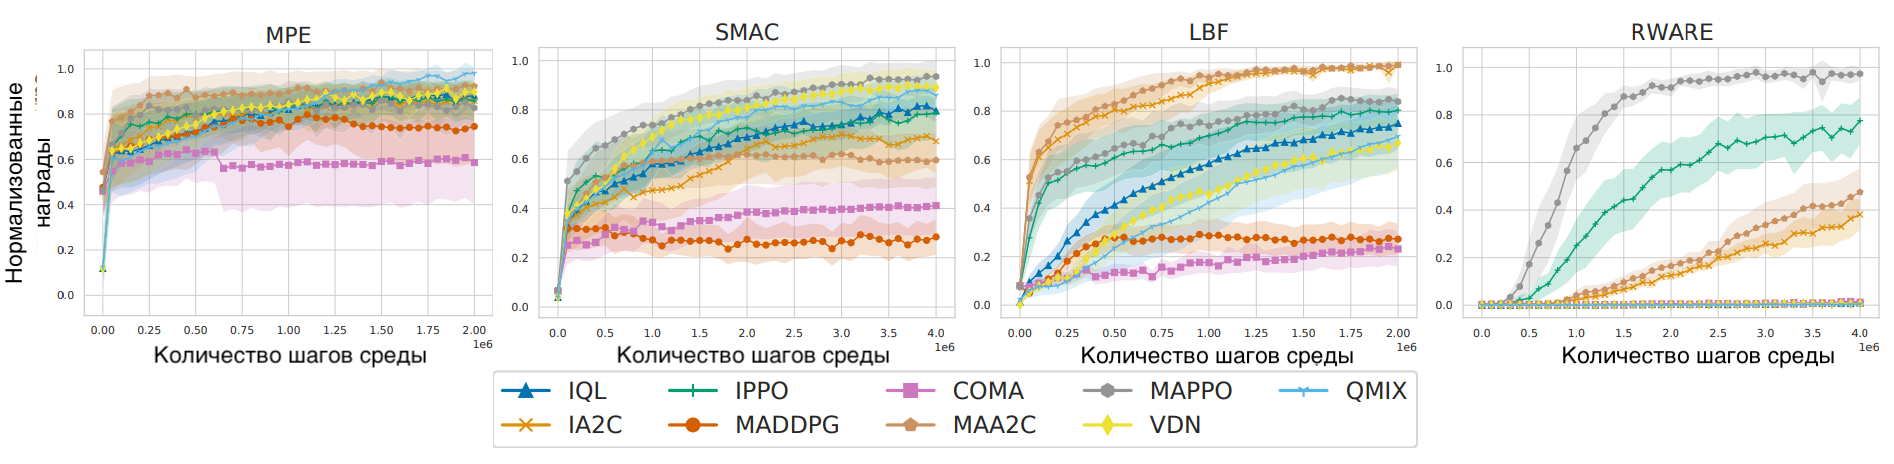
\includegraphics[pages=-, width=140mm]{./inc/img/comp_big.png}
	\caption{Нормализованное вознаграждение разных алгоритмов в на разных средах в зависимости от кол--ва эпизодов для обучения}
	\label{fig:mappo_perf}
\end{center}
\end{figure}

\ref{fig:mappo_perf} \cite{DBLP:journals/corr/abs-2103-01955} включает в себя все рассматриваемые игры. Можно сделать вывод, что MAPPO показывает лучшие результаты в большинстве сред.
IPPO, не включающий в себя методы обучения нескольких агентов, показывает хорошие результаты в большинстве сред. Это было подмечено в статье \cite{DBLP:journals/corr/abs-2103-01955}.

Модификации классических алгоритмов для среды с несколькими агентами показывают средние результаты, за исключением среды IBF где A2C (как обычный вариант, так и с централизованным обучением Q) показывает наилучшие результаты. 

\subsection*{Вывод}

Была предложена метрика сравнения алгоритмов (по средней награде в игре, по проценту побед, по нормализованной средней награде), приведены графики сравнения алгоритмов по выбранной метрике. Даны комментарии к графикам, советы по выбору того или иного алгоритма.
Можно считать, что обсуждаемые результаты достоверны, исходя из открытых инструментов для сравнения.

